\chapter{Codifica}

Questo capitolo tratta gli aspetti più interessanti della codifica dell'applicazione moviORDER. In particolare, il capitolo è stato diviso in sezioni che trattano la codifica di:
\begin{enumerate}
	\item \textbf{servizio web};
	\item \textbf{logica applicativa};
	\item \textbf{interfaccia grafica}.
\end{enumerate}

\section{Servizio web}

Per lo sviluppo del servizio web che permette all'applicazione di accedere al database presente sul server cloud di \visione{} si è utilizzato il linguaggio Java e, nello specifico, gli oggetti servlet. Per permettere agli oggetti servlet di interagire con il database si sono dovuti utilizzare i driver JDBC per SQL Server, in quanto moviORDER è basata su tale database. 

\subsection{Servlet}

In questa sezione viene presentato l'utilizzo degli oggetti servlet nella realizzazione del servizio web.

\subsubsection{Struttura di un oggetto servlet}

Un oggetto servlet è una classe Java che eredita dalla classe \textit{HttpServlet}, appartenente al package \textit{javax.servlet.http}. \textit{HttpServlet} è una classe astratta che può essere estesa per creare un servlet HTTP utilizzabile per un sito web. Nel progetto realizzato, il servlet è stato utilizzato per acquisire richieste HTTP POST, per elaborarle interrogando il database sul server cloud di \visione{}, e per rispondere ad esse tramite una stringa in formato JSON. Ogni servlet del servizio web implementa il metodo \textit{protected void doPost(HttpServletRequest req, HttpServletResponse resp)}. Tale metodo viene chiamato dal server per permettere all'oggetto servlet di acquisire una richiesta POST da parte di un client. Nel caso del progetto, il client è la logica applicativa dell'applicazione moviORDER e il server è Apache Tomcat.

\textit{HttpServletRequest} è la classe Java che rappresenta le richieste HTTP che possono essere inviate all'oggetto servlet. Tramite opportuni metodi è possibile accedere alle informazioni contenute nella specifica richiesta. Tramite il metodo \textit{String getParameter(String name)} è possibile, data una stringa rappresentante un parametro della richiesta HTTP, ottenere una stringa contenente il valore associato a tale parametro, oppure il valore \textit{null} se il parametro non esiste.

\textit{HttpServletResponse} è la classe Java che rappresenta la risposta dell'oggetto servlet alla richiesta del client. Tramite opportuni metodi è possibile configurare la risposta:
\begin{itemize}
	\item \textit{void setContentType(String type)}: permette di impostare la tipologia di contenuto della risposta. Nel progetto la risposta è una stringa in formato JSON, quindi è stato impostato il content type \textit{application/json};
	\item \textit{PrintWriter getWriter()}: restituisce un oggetto \textit{PrintWriter} che può essere utilizzato per inviare caratteri di testo al client. Nel progetto, l'oggetto \textit{PrintWriter} è stato utilizzato per inviare la stringa di risposta in formato JSON.
\end{itemize}

Viene di seguito fornita, a titolo d'esempio, l'implementazione del metodo \textit{doPost()} del servlet del servizio web che si occupa di controllare che le credenziali inserite dall'utente in fase di login siano corrette. Nella prossima sezione viene fornito un esempio di come la logica applicativa di moviORDER effettua una richiesta a tale servlet e di come utilizza la risposta per modificare lo stato dell'applicazione. Nell'esempio, la classe \textit{DatabaseConnection} fornisce un'interfaccia per l'interrogazione di un database SQL Server. Una spiegazione di tale classe è presente in sezione \ref{dbconnect}.

\begin{figure}[!h] 
    \centering 
    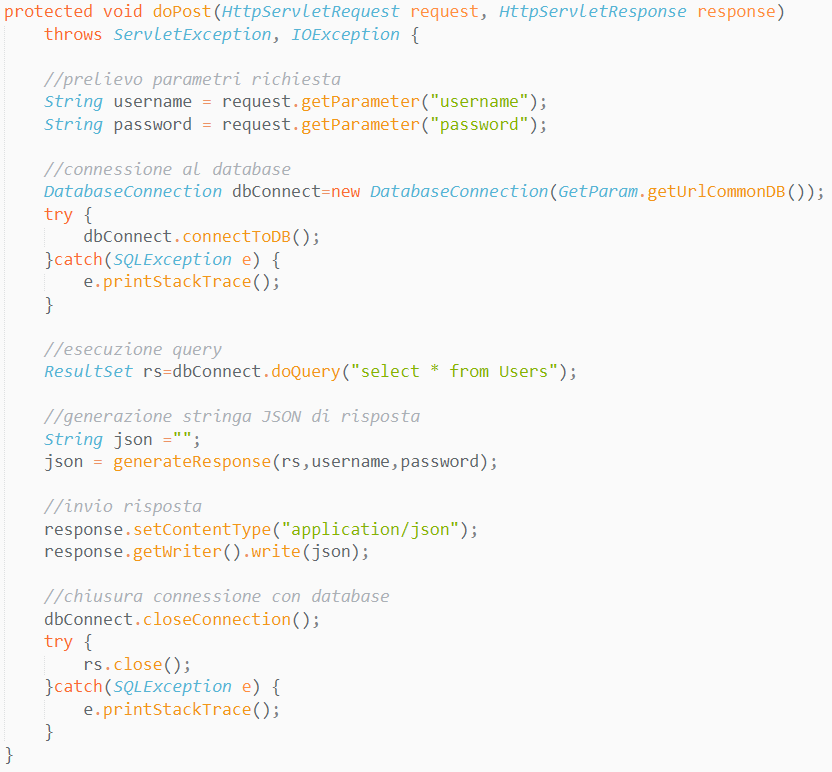
\includegraphics[height=10cm,width=\columnwidth]{codice/servlet} 
    \caption{Metodo \textit{doPost()} del servlet che gestisce l'autenticazione}
\end{figure}

\subsubsection{Interrogazione del servizio web}

Nel momento in cui viene implementato un servlet concreto, eclipse gli associa un end-point in automatico. Tramite l'end-point è possibile raggiungere il servlet sul server per effettuare richieste HTTP. L'end-point associato da eclipse è della forma \textit{/NomeClasseServlet} e puo' essere cambiato dalle impostazioni dell'IDE. Per rendere possibile il raggiungimento del servizio web da parte della logica applicativa di moviORDER, è necessario che venga effettuato il deploy del servizio su Apache Tomcat e che quest'ultimo venga fatto girare sul server cloud di \visione{}. Una volta che il servizio web è raggiungibile tramite la rete, è possibile iniziare ad effettuare richieste HTTP. In moviORDER, la struttura dell'URL di una richiesta HTTP è la seguente: \textit{http://indirizzo:porta/moviORDER/NomeServlet}, dove:
\begin{itemize}
	\item \textit{indirizzo}: è l'indirizzo del server dove il servizio web viene fatto girare:
	\item \textit{porta}: è la porta del server dove il servizio web viene fatto girare;
	\item \textit{NomeServlet}: è l'end-point (servlet) a cui si vuole inviare la richiesta HTTP.
\end{itemize}

MoviORDER effettua richieste HTTP tramite l'utilizzo di AJAX (Asynchronous JavaScript And XML). È importante far notare che AJAX non è un linguaggio di programmazione, bensì una tecnica per accedere ad un server web da una pagina web. Tramite AJAX è possibile leggere dati da un server web dopo che una pagina è stata caricata, aggiornare una pagina web senza il bisogno di dover ricaricare la stessa e inviare dati ad un server web in maniera del tutto trasparente all'utente. 

Nel progetto, AJAX è stato implementato mediante JavaScript con l'utilizzo dell'oggetto \textit{XMLHttpRequest}. Tale oggetto è supportato da tutti i browser moderni e può essere utilizzato per scambiare dati con un server web in maniera trasparente, ovvero senza il bisogno di dover ricaricare la pagina web per cambiarne lo stato. La sintassi per la creazione di un oggetto \textit{XMLHttpRequest} è la seguente:
\textit{var xhttp = new XMLHttpRequest();}. 

Per l'invio di richieste HTTP al servizio web si utilizzano i metodi \textit{open()} e \textit{send()} di \textit{XMLHttpRequest}. In particolare, il metodo \textit{open()} permette di specificare la tipologia di richiesta tramite il passaggio di tre parametri:
	\begin{itemize}
		\item \textbf{metodo}: specifica il metodo utilizzato per inviare la richiesta HTTP: GET o POST;
		\item \textbf{url}: specifica l'indirizzo del server a cui inviare la richiesta HTTP. Nel caso del progetto l'indirizzo comprende l'end-point presso il quale la richiesta deve essere gestita;
		\item \textbf{asincrona/sincrona}: specifica se la richiesta è asincrona (true) o sincrona (false).
	\end{itemize}
Il metodo \textit{send(string)} permette invece l'invio di una richiesta HTTP al servizio web. Esso richiede il passaggio di una stringa contenente i parametri da inviare al server. Poiché alcuni parametri possono contenere caratteri accentati, è stato necessario utilizzare il metodo \textit{setRequestHeader()} per specificare la codifica dei caratteri, aggiungendo header HTTP alla richiesta. Facendo questo, è stato possibile evitare errori di lettura/scrittura di stringhe con caratteri accentati sul database di moviORDER. 

È importante far notare che tutte le richieste HTTP inviate da moviORDER al servizio web sono asincrone, questo perché:
\begin{itemize}
	\item il codice sincrono non è raccomandato poiché JavaScript stopperebbe l'esecuzione fino all'arrivo di una risposta da parte del server. Se il server è occupato o lento, l'applicazione potrebbe aspettare per un tempo prolungato;
	\item le richieste AJAX di tipo sincrono saranno rimosse dallo standard web nei prossimi anni. Scegliendo di utilizzare solamente richieste asincrone si permette a moviORDER di essere robusta a questo cambiamento futuro.
\end{itemize} 

Per la gestione della risposta ricevuta dal server si sono utilizzate le seguenti proprietà dell'oggetto \textit{XMLHttpRequest}:
\begin{itemize}
	\item \textit{readyState}: contiene lo stato dell'oggetto. In particolare, per lo scopo del progetto, è interessante sapere che il valore 4 corrisponde ad una richiesta la cui risposta è pronta;
	\item  \textit{status}: contiene il messaggio sullo stato della richiesta. In particolare, per lo scopo del progetto, è interessante sapere che il valore 200 corrisponde al messaggio OK, che nello standard web rappresenta una richiesta HTTP andata a buon fine;
	\item \textit{onreadystatechange}: definisce una funzione che deve essere eseguita quando la proprietà \textit{readyState} cambia valore;
	\item \textit{responseText}: incapsula la stringa di risposta ricevuta dal servizio web. 
\end{itemize} 
Poiché la risposta ricevuta dal servizio web è una stringa in formato JSON, per effettuare il parsing di tale stringa è stato necessario convertirla in un oggetto JavaScript, tramite l'utilizzo del metodo \textit{JSON.parse()}.

Viene di seguito fornito, a titolo d'esempio, il codice JavaScript della logica applicativa di moviORDER che effettua una chiamata HTTP all'end-point (servlet) che si occupa di gestire l'autenticazione. Il codice si occupa anche di gestire la risposta ricevuta dal servizio web. La funzione \textit{tryLogin()} viene eseguita nel momento in cui l'utente preme sul pulsante di login presente nella schermata di login dell'applicazione.

\newpage

\begin{figure}[!h] 
    \centering 
    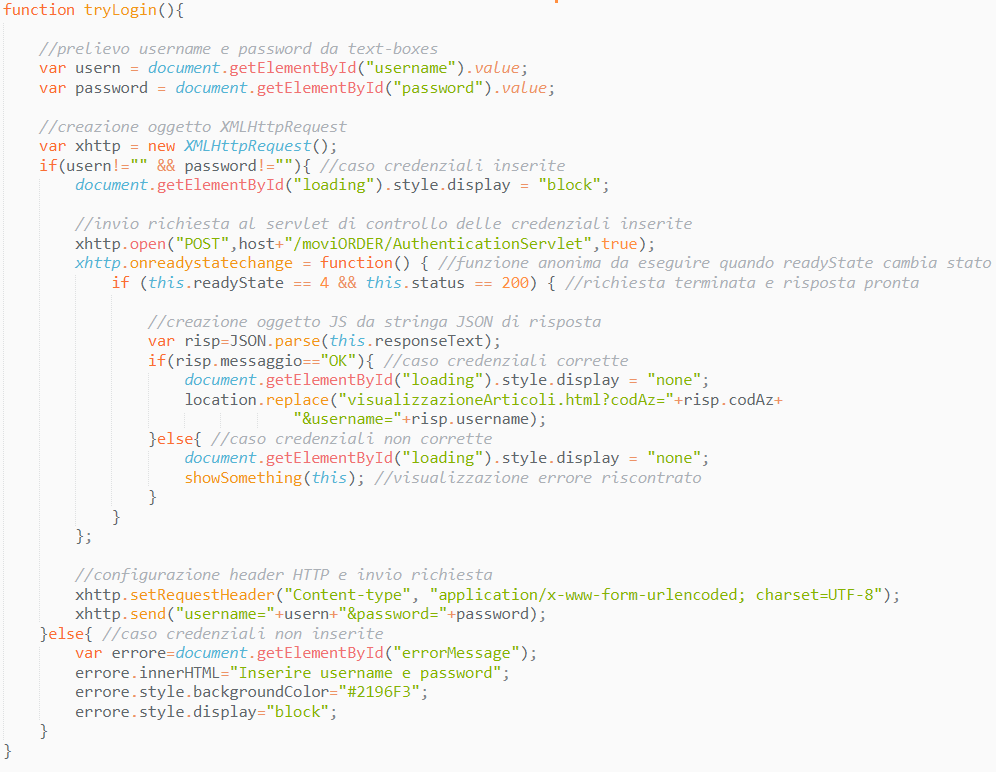
\includegraphics[width=\columnwidth]{codice/ajax} 
    \caption{Esempio di invio di una richiesta HTTP tramite AJAX}
\end{figure}

\subsubsection{API del servizio web} \label{api}

In questa sezione viene presentata la API del servizio web di moviORDER. In particolare, per ogni end-point (servlet) vengono specificati:
\begin{itemize}
	\item \textbf{indirizzo}: indirizzo tramite il quale è possibile raggiungere l'end-point;
	\item \textbf{input}: costituito dai parametri inviati al servizio web tramite una richiesta HTTP;
	\item \textbf{output}: costituito da una stringa in formato JSON che presenta struttura diversa a seconda dell'end-point che gestisce la richiesta;
	\item \textbf{descrizione}.
\end{itemize}

\myparagraph{Servizio di autenticazione}

\begin{itemize}
	\item \textbf{Indirizzo}: /AuthenticationServlet;
	\item \textbf{Input}:
		\begin{itemize}
			\item \textit{username}: è la username inserita dall'utente in fase di login;
			\item \textit{password}: è la password inserita dall'utente in fase di login.
		\end{itemize}
	\item \textbf{Output}: le possibili risposte del servlet sono le seguenti:
		\begin{itemize}
			\item codice azienda e username dell'utente nel caso in cui username e password corrispondano ad un utente presente in database;
			\item un messaggio d'errore nel caso in cui username e password siano scorrette o l'utente è stato bloccato. 
		\end{itemize}
		\item \textbf{Descrizione}: questo servlet rappresenta il servizio di autenticazione di moviORDER. Ricevuti i parametri, il servlet cerca la username dell'utente nel database e, nel caso in cui questa fosse presente, procede nel cercare la password corrispondente. Nel caso in cui username e password passati siano quelli corretti, il servlet restituisce una stringa JSON contenente il codice azienda e la username dell'utente che ha cercando di loggarsi. Nel caso in cui le credenziali non siano corrette, oppure l'utente è stato bloccato, viene restituito un messaggio d'errore.
\end{itemize}

\myparagraph{Servizio di verifica di connessione con il database}

\begin{itemize}
	\item \textbf{Indirizzo}: /CheckConnectionURL;
	\item \textbf{Input}:
		\begin{itemize}
			\item codice azienda: è il codice azienda dell'azienda cliente di \visione{} della quale si vuole verificare la presenza del database.
		\end{itemize}
	\item \textbf{Output}: le possibili risposte del servlet sono le seguenti:
		\begin{itemize}
			\item un messaggio positivo nel caso in cui il database dell'azienda corrispondente al codice inserito sia raggiungibile;
			\item un messaggio negativo nel caso in cui il database dell'azienda corrispondente al codice inserito non sia raggiungibile.
		\end{itemize}
	\item \textbf{Descrizione}: questo servlet si occupa di controllare se un database aziendale è raggiungibile effettuando una query su tale database. Risponde positivamente nel caso in cui il database dell'azienda corrispondente al codice inserito fosse raggiungibile (query con un ritorno), mentre risponde negativamente nel caso in cui il database non fosse raggiungibile (query che ha sollevato un eccezione).
\end{itemize}

\myparagraph{Servizio di rimozione articoli dal carrello}

\begin{itemize}
	\item \textbf{Indirizzo}: /DeleteSelectedItems;
	\item \textbf{Input}:
		\begin{itemize}
			\item lista di codici articolo: è una lista di dei codici articolo degli articoli che devono essere eliminati;
			\item username: è la username dell'utente che ha richiesto l'eliminazione degli articoli;
			\item path: è la stringa di connessione al database aziendale dell'utente autenticato.
		\end{itemize}
	\item \textbf{Output}: le possibili risposte del servlet sono le seguenti:
		\begin{itemize}
			\item un messaggio positivo nel caso in cui la cancellazione sia andata a buon fine;
			\item un messaggio negativo nel caso in cui la cancellazione non sia andata a buon fine.
		\end{itemize}
	\item \textbf{Descrizione}: questo servlet si occupa di eliminare dal database aziendale dell'utente autenticato gli articoli che l'utente ha richiesto di rimuovere dal carrello. Risponde positivamente nel caso in cui gli articoli sono stati rimossi correttamente dal database, mentre risponde negativamente nel caso in cui gli articoli non sono stati rimossi dal database.
\end{itemize}

\myparagraph{Servizio di ricerca di un codice a barre}

\begin{itemize}
	\item \textbf{Indirizzo}: /FindArticleBarCode;
	\item \textbf{Input}:
		\begin{itemize}
			\item codice a barre: è il codice a barre di un articolo del quale si vuole conoscere il codice articolo;
			\item path: è la stringa di connessione al database aziendale dell'utente autenticato.
		\end{itemize}
	\item \textbf{Output}: le possibili risposte del servlet sono le seguenti:
		\begin{itemize}
			\item codice articolo corrispondente al barcode passato come parametro nel caso in cui il barcode corrisponda a quello di un articolo venduto dall'azienda;
			\item un messaggio negativo nel caso in cui il barcode passato come parametro non corrisponda ad un articolo venduto dall'azienda.
		\end{itemize}
	\item \textbf{Descrizione}: questo servlet si occupa di fornire il codice articolo dell'articolo corrispondente al codice a barre ricevuto come parametro, effettuando la ricerca del barcode all'interno del database. Nel caso in cui il codice a barre sia presente all'interno del database viene restituito il codice articolo corrispondente, mentre nel caso in cui non fosse presente viene restituito un messaggio negativo.
\end{itemize}

\myparagraph{Servizio di ricerca di un codice articolo}

\begin{itemize}
	\item \textbf{Indirizzo}: /FindArticleCode;
	\item \textbf{Input}:
		\begin{itemize}
			\item codice articolo: è il codice articolo o il barcode di un articolo del quale si vuole verificare la presenza in database;
		\end{itemize}
	\item \textbf{Output}: le possibili risposte del servlet sono le seguenti:
		\begin{itemize}
			\item codice articolo nel caso in cui l'articolo sia presente in database;
			\item un messaggio negativo nel caso in cui l'articolo non sia presente in database.
		\end{itemize}
	\item \textbf{Descrizione}: questo servlet si occupa di fornire il codice articolo dell'articolo corrispondente al codice articolo o al barcode ricevuto come parametro, effettuando la ricerca del codice articolo all'interno del database. Nel caso in cui il codice articolo o il barcode passato come parametro corrisponda ad un articolo presente in database viene restituito il codice articolo dell'articolo, mentre nel caso in cui non corrisponda ad un articolo presente in database viene restituito un messaggio negativo.
\end{itemize}

\myparagraph{Servizio di prelievo informazioni di un articolo}

\begin{itemize}
	\item \textbf{Indirizzo}: /GetArticleDescNote;
	\item \textbf{Input}:
		\begin{itemize}
			\item codice azienda: è il codice azienda della quale l'utente autenticato è cliente;
			\item codice articolo: è il codice articolo dell'articolo del quale si vogliono ottenere informazioni.
		\end{itemize}
	\item \textbf{Output}: questo servlet può produrre un solo output perché l'applicazione è stata implementata in modo che non ci siano casi negativi:
		\begin{itemize}
			\item descrizione, note, quantità minima ordinabile e step di quantità permessi per l'articolo corrispondente al codice articolo passato come parametro.
		\end{itemize}
	\item \textbf{Descrizione}: questo servlet si occupa di fornire informazioni sull'articolo corrispondente al codice articolo passato come parametro. 
\end{itemize}

\myparagraph{Servizio di prelievo degli articoli nel carrello di un utente}

\begin{itemize}
	\item \textbf{Indirizzo}: /GetArticlesByUsername;
	\item \textbf{Input}:
		\begin{itemize}
			\item codice azienda: è il codice azienda della quale l'utente autenticato è cliente;
			\item username: è il nome utente dell'utente autenticato.
		\end{itemize}
	\item \textbf{Output}: le possibili risposte del servlet sono le seguenti:
		\begin{itemize}
			\item array degli articoli nel carrello dell'utente autenticato. Per ogni articolo vengono restituiti la quantità ordinata, il codice articolo e la descrizione dell'articolo;
			\item array vuoto nel caso in cui l'utente autenticato non presenti articoli in carrello.
		\end{itemize}
	\item \textbf{Descrizione}: questo servlet si occupa di fornire la lista di articoli in carrello per l'utente la quale username è stata passata come parametro. Nel caso in cui l'utente presenti articoli in carrello viene restituita la lista degli articoli in carrello, mentre nel caso in cui non presenti articoli in carrello viene restituita una lista vuota.
\end{itemize}

\myparagraph{Servizio di prelievo di informazioni di un utente}

\begin{itemize}
	\item \textbf{Indirizzo}: /GetNameByUsername;
	\item \textbf{Input}:
		\begin{itemize}
			\item path: è la stringa di connessione al database aziendale dell'utente autenticato;
			\item username: è il nome utente dell'utente autenticato.
		\end{itemize}
	\item \textbf{Output}: questo servlet può produrre un solo output perché l'applicazione è stata implementata in modo che non ci siano casi negativi:
		\begin{itemize}
			\item nome e ragione sociale dell'utente autenticato e codice documento e descrizione del documento da generare nel caso in cui l'utente invii un ordine.
		\end{itemize}
	\item \textbf{Descrizione}: questo servlet si occupa di fornire informazioni sull'utente la cui username è stata passata come parametro.
\end{itemize}

\myparagraph{Servizio di prelievo informazioni di un articolo in carrello}

\begin{itemize}
	\item \textbf{Indirizzo}: /GetTmpArticleData;
	\item \textbf{Input}:
		\begin{itemize}
			\item path: è la stringa di connessione al database aziendale dell'utente autenticato;
			\item codice articolo: è il codice articolo dell'articolo del quale si vogliono ottenere informazioni;
			\item username: è il nome utente dell'utente autenticato.
		\end{itemize}
	\item \textbf{Output}: questo servlet può produrre un solo output perché l'applicazione è stata implementata in modo che non ci siano casi negativi:
		\begin{itemize}
			\item quantità e note dell'articolo nel carrello dell'utente autenticato corrispondente al codice articolo passato come parametro.
		\end{itemize}
	\item \textbf{Descrizione}: questo servlet si occupa di fornire informazioni riguardati uno specifico articolo nel carrello dell'utente la quale username è stata passata come parametro.
\end{itemize}

\myparagraph{Servizio di inserimento/modifica articolo}

\begin{itemize}
	\item \textbf{Indirizzo}: /InsertUpdateArticle;
	\item \textbf{Input}:
		\begin{itemize}
			\item path: è la stringa di connessione al database aziendale dell'utente autenticato;
			\item query: è la query di inserimento/modifica di un articolo.
		\end{itemize}
	\item \textbf{Output}: le possibili risposte del servlet sono le seguenti:
		\begin{itemize}
			\item un messaggio positivo nel caso in cui la query di inserimento/modifica articolo sia andata a buon fine;
			\item un messaggio negativo nel caso in cui la query di inserimento/modifica articolo non sia andata a buon fine.
		\end{itemize}
	\item \textbf{Descrizione}: questo servlet si occupa di inserire o modificare un articolo nel carrello dell'utente autenticato. L'inserimento e la modifica avvengono mediante l'utilizzo dello stesso servlet poiché uno dei parametri è la query da eseguire sul database, che può essere di tipo INSERT o UPDATE. Nel caso in cui la query venga eseguita in modo corretto sul database viene restituito un messaggio positivo, mentre nel caso in cui non venga eseguita viene restituito un messaggio negativo.
\end{itemize}

\myparagraph{Servizio di invio di un ordine}

\begin{itemize}
	\item \textbf{Indirizzo}: /SendOrder;
	\item \textbf{Input}:
		\begin{itemize}
			\item path: è la stringa di connessione al database aziendale dell'utente autenticato;
			\item codici articolo: è la lista dei codici degli articoli che l'utente autenticato ha ordinato;
			\item username: è il nome utente dell'utente autenticato;
			\item ragione sociale: è la ragione sociale dell'utente autenticato;
			\item nome: è il nome dell'utente autenticato;
			\item codice documento: è il codice del documento che deve essere generato con l'ordine;
			\item data: è la data d'invio dell'ordine;
			\item note: sono le note inserite dall'utente in fase di invio dell'ordine;
			\item codice azienda: è il codice azienda della quale l'utente autenticato è cliente.
		\end{itemize}
	\item \textbf{Output}: le possibili risposte del servlet sono le seguenti:
		\begin{itemize}
			\item un messaggio positivo nel caso in cui l'ordine sia stato inviato con successo;
			\item un messaggio negativo nel caso in cui l'ordine non sia stato inviato con successo.
		\end{itemize}
	\item \textbf{Descrizione}: questo servlet si occupa di registrare in database un ordine contenente gli articoli passati come parametro. Il resto dei parametri che vengono passati viene utilizzato per inviare una mail di conferma all'utente autenticato e all'azienda presso cui l'utente è cliente. Nel caso in cui la registrazione dell'ordine in database avvenga correttamente viene restituito un messaggio positivo, mentre nel caso in cui non avvenga correttamente viene restituito un messaggio negativo.
\end{itemize}

\subsection{JDBC}

In questa sezione viene presentato l'utilizzo della Java Database Connectivity API nella realizzazione del servizio web.

\subsubsection{Driver JDBC}

Un driver JDBC è una componente software che permette ad un'applicazione Java di interagire con un database. Per supportare la connessione a singoli database, JDBC (Java Database Connectivity API) richiede i driver per ogni database. Il driver permette la connessione con il database e implementa il protocollo di trasferimento di query e risultati tra il client e il database. Poiché per l'implementazione del database è stato utilizzato SQL Server si sono dovuti utilizzare i driver JDBC per tale database.

\subsubsection{Classe DatabaseConnection} \label{dbconnect}

Per lo sviluppo del servizio web è stata realizzata la classe \textit{DatabaseConnection} appartenente al package \textit{dbConnection}. Tale classe fornisce un'interfaccia utilizzabile per la gestione dell'interazione con un database di tipo SQL Server. In questa sezione vengono presentati i metodi che costituiscono tale interfaccia.

\myparagraph{Costruttori}

La classe presenta due metodi costruttori:
\begin{itemize}
	\item \textit{public DatabaseConnection(String u, String user, String psw, String db)}: costruisce un oggetto \textit{DatabaseConnection} a partire dall'URL del server in cui è presente il database, la username e la password di accesso al database, e il nome del database al quale si desidera connettesi;
	\item \textit{public DatabaseConnection(String dbConnectionString)}: costruisce un oggetto \textit{DatabaseConnection} a partire dalla stringa di connessione ad uno specifico database.
\end{itemize}
Il formato della stringa di connessione ad un database è il seguente: \textit{indirizzoServer;databaseName=nomeDb;user=u;password=psw}, dove:
\begin{itemize}
	\item \textit{indirizzoServer}: è l'indirizzo IP pubblico del server contenente il database al quale si desidera connettersi. Nel caso del progetto potrebbe essere l'indirizzo del server di un'azienda esterna che desidera utilizzare il proprio database per l'interazione;
	\item \textit{nomeDb}: è il nome del database al quale si desidera connettersi;
	\item \textit{u}: è il nome utente per l'accesso al database;
	\item \textit{psw}: è la password per l'accesso al database.
\end{itemize}
Viene di seguito presentato, a titolo d'esempio, il codice Java che implementa il metodo \textit{public DatabaseConnection(String dbConnectionString)}. Il metodo si occupa di splittare la stringa di connessione passata come parametro per ottenere i dati utili alla costruzione dell'oggetto \textit{DatabaseConnection}.

\begin{figure}[!h] 
    \centering 
    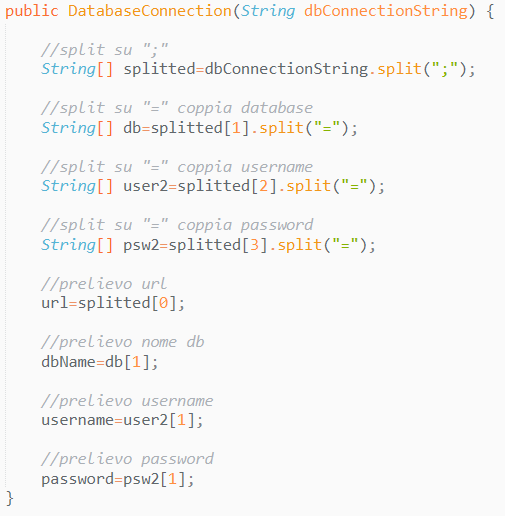
\includegraphics[height=8cm,width=0.8\columnwidth]{codice/databaseCostruttore} 
    \caption{Metodo costruttore della classe \textit{DatabaseConnection}}
\end{figure}

\myparagraph{Metodo \textit{connectToDb()}}

Tale metodo si occupa di instaurare la connessione con il database desiderato. Per far questo, configura i driver JDBC e costruisce l'URL di connessione al database tramite i dati contenuti nell'oggetto d'invocazione. Il metodo potrebbe sollevare un'eccezione di tipo \textit{ClassNotFoundException} nel caso in cui la classe utilizzata per i driver JDBC sia inesistente o non sia stata importata all'interno del progetto. Viene di seguito fornito, a titolo d'esempio, il codice del metodo \textit{connectToDb()}.

\begin{figure}[!h] 
    \centering 
    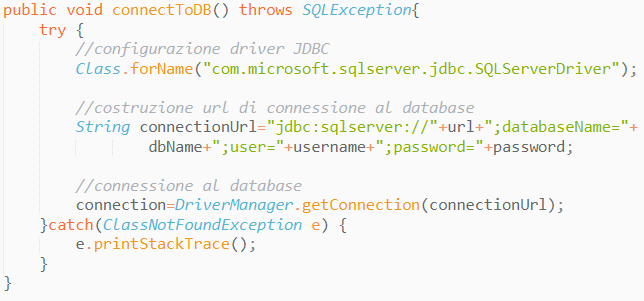
\includegraphics[width=\columnwidth]{codice/connessionedb} 
    \caption{Metodo \textit{connectToDb()} della classe \textit{DatabaseConnection}}
\end{figure}

\myparagraph{Altri metodi}

Sono stati implementati altri metodi di complessità inferiore. Per questo motivo ne viene presentata solamente una breve descrizione:
\begin{itemize}
	\item \textit{doQuery(query)}: questo metodo permette di eseguire una query di tipo SELECT sul database. Restituisce il \textit{ResultSet} contenente il risultato della query;
	\item \textit{doUpdateQuery(query)}: questo metodo permette di eseguire una query di tipo INSERT, UPDATE o DELETE sul database. Restituisce il numero di righe inserite, modificate o cancellate;
	\item \textit{closeConnection()}: questo metodo permette di eseguire il processo di disconnessione dal database.
\end{itemize}

\subsection{Classi utilità}

Per lo sviluppo del servizio web è stato necessario implementare due classi utilità. In questa sezione ne viene presentata brevemente l'implementazione. Tali classi appartengono al package \textit{utility}.

\subsubsection{Classe GetParam}

La classe \textit{GetParam} si occupa di restituisce un campo statico contenente la stringa di connessione al database \textit{CommonDb} dell'applicazione moviORDER. Come detto precedentemente, questo database contiene tutti i dati di autenticazione degli utenti di moviORDER. Poiché tale stringa di connessione viene utilizzata frequentemente all'interno del servizio web, si è deciso di inserirla in un unico punto del servizio, in modo da evitare la modifica di più file nel caso in cui essa cambi.

\subsubsection{Classe MailUtility}

La classe \textit{MailUtility} fornisce un'interfaccia per l'invio di e-mail. È stato necessario implementare tale classe poiché è stato richiesto di inviare una mail di conferma all'utente autenticato e all'azienda presso cui l'utente è cliente nel momento in cui un ordine viene registrato. La classe presenta un costruttore che richiede i parametri per la configurazione di un server SMTP:
\begin{itemize}
	\item \textbf{host}: è l'indirizzo IP dell'host su cui è installato il server SMTP;
	\item \textbf{post}: è il numero di porta dell'host su cui è installato il server SMTP;
	\item \textbf{username}: è il nome utente di accesso al server SMTP;
	\item \textbf{password}: è la password di accesso al server SMTP.
\end{itemize}
Il metodo \textit{sendMail()} si occupa di configurare e inviare una mail all'utente che ha effettuato l'ordine e all'azienda presso cui l'utente è cliente. Per far questo, il metodo richiede:
\begin{itemize}
	\item indirizzo e-mail dell'utente;
	\item indirizzo e-mail dell'azienda;
	\item indirizzo e-mail del mittente;
	\item oggetto della e-mail;
	\item testo della e-mail: è una tabella scritta in codice HTML contenente i dati degli articoli ordinati.
\end{itemize}
Viene di seguito fornito, a titolo d'esempio, il codice Java che implementa il metodo \textit{sendMail()}.

\begin{figure}[!h] 
    \centering 
    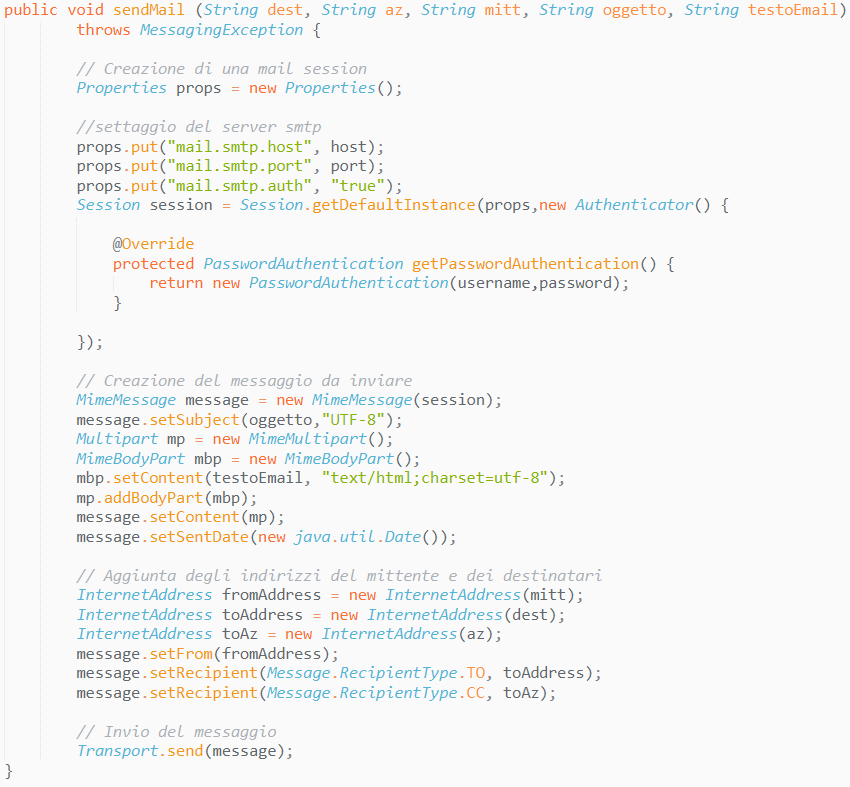
\includegraphics[width=\columnwidth]{codice/mail} 
    \caption{Metodo \textit{sendMail()} della classe \textit{MailUtility}}
\end{figure}

\section{Logica applicativa}

Parlare dei plugin di phonegap e fare l'esempio del barcode scanner, parlare degli alert come permettono di essere convertiti in nativo e di tutte queste cose sui plugin. Aspetti negativi e positivi dei plugin nelle varie piattaforme, se funzionano allo stesso modo o ci sono state delle differenze sostanziali.

\section{Interfaccia grafica}

mostrare lo screen delle varie interfacce e spiegarne le interazioni utente

\textbf{per la parte di progettazione far vedere che il database potrebbe essere anche sul server di un'azienda esterna, commonDB sempre sul server vision mentre il db dell'azienda può essere su un server esterno.}
